\chapter{Einführung und Fragestellung}
In der Robotik, in der Roboter mit möglichst wenig Zutun von außen arbeiten sollen, spielt die künstliche Intelligenz eine wichtige Rolle. Das Vorhandensein der Intelligenz bei Robotern könnte für einen höheren Grad an Automatisierung sorgen. Eine Maschine oder ein Roboter muss dann beispielsweise nicht für einen speziellen Fall ausgelegt sein, zum Beispiel das Erkennen des Gesichts einer bestimmten Person, sondern ist \textit{intelligent} und kann die Gesichter sämtlicher Personen identifizieren. 
Da die Themen \textit{künstliche Intelligenz} und \textit{maschinelles Lernen} bisher kein Gegenstand einer Vorlesung waren, an denen der Autor teilgenommen hat, erfolgt zunächst ein grober Überblick über diese Themen.
Anschließend wird gezeigt, was Bayes'sche Netze sind und für was man sie in der Robotik verwenden kann.\begin{figure}%[h!]
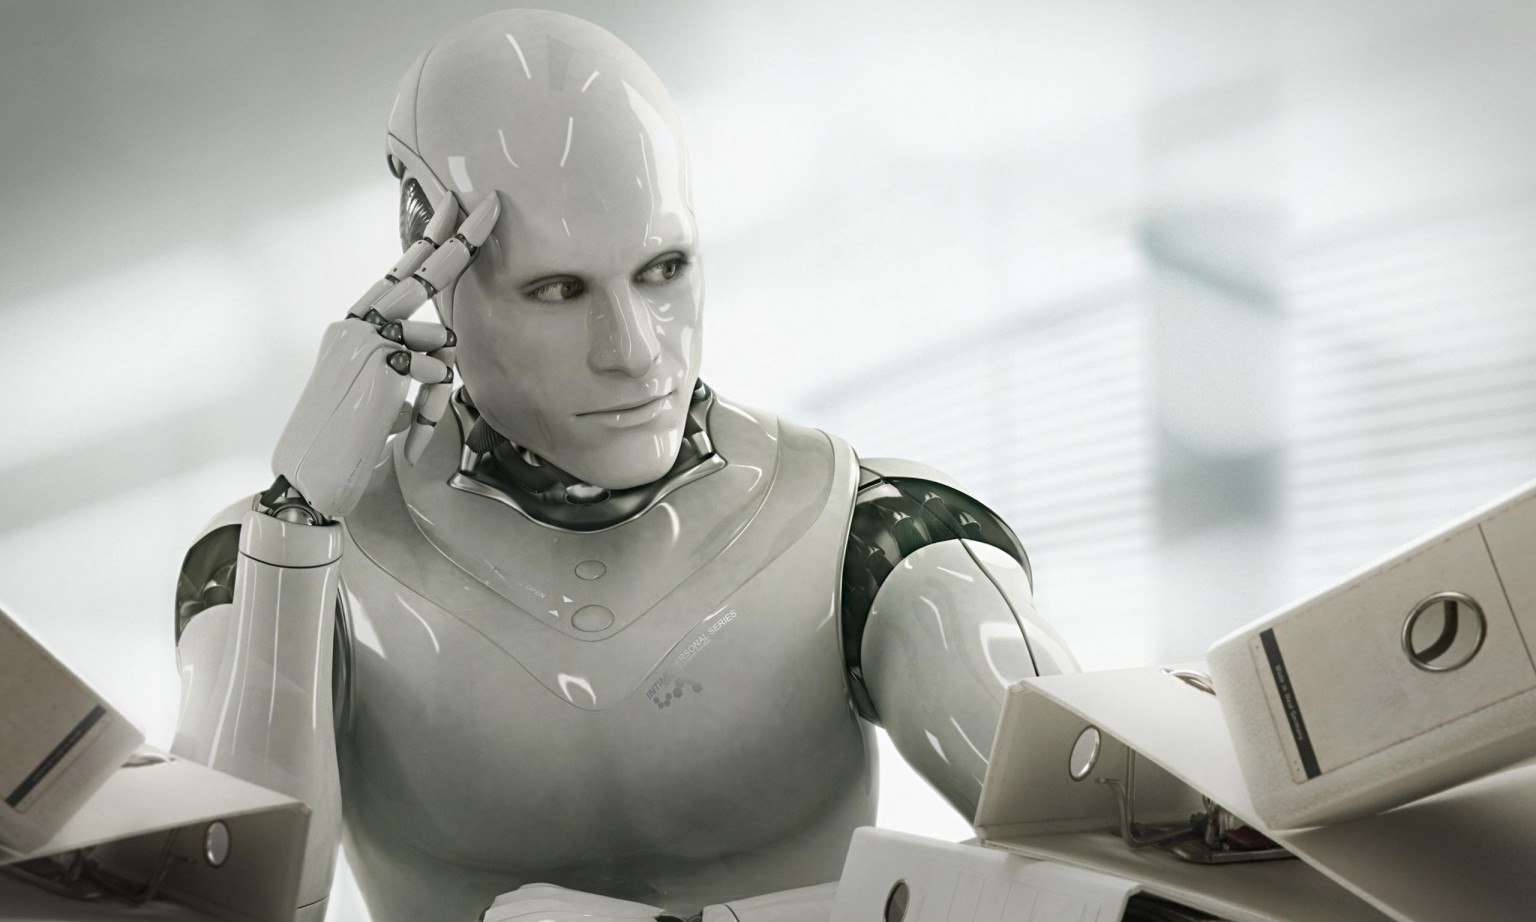
\includegraphics[scale=0.15]{bilder/RobotTakeOverBS} 
\caption{Robot take over \cite{venturesafrica}}
\label{Entdeckungswahrscheinlichkeit}
\end{figure}
